\chapter{Models, memory and observation}\label{ch:models}

The central difficulty is to separate three objects that are often conflated in stress-release modelling: the physical state that carries memory, the point process that records event occurrence, and the observation model through which events and their marks become data. The finite-mode formulation provides a transparent autonomous physical model. A diagnostic formulation specifies an independent background and separates its suppression from triggering. The distinction matters because stability, approximation and inference make different demands on the model.

\section{The physical finite-mode model}\label{sec:model_physical}

Let \(\vartheta_j>0\) be relaxation rates and let \(w_j>0\), \(\sum_jw_j=1\), be fixed weights. For a constant loading \(\rho\geq0\), write
\[
x_j^*=\frac{\rho}{\vartheta_j},\qquad
\bar x=\sum_jw_jx_j^*,\qquad
\mathcal X=\left\{(Z,U):Z_j\leq x_j^*,\ U_j\geq0\right\}.
\]
The physical stress and excitation reservoir are
\begin{equation}\label{eq:physical-XH}
X=\sum_jw_jZ_j,\qquad H=\sum_jw_jU_j.
\end{equation}
Between events the coordinates relax according to
\begin{equation}\label{eq:finite-flow}
\dot Z_j=\rho-\vartheta_jZ_j,\qquad
\dot U_j=-\vartheta_jU_j.
\end{equation}
The ground event process \(N\) has compensator
\begin{equation}\label{eq:physical-compensator}
\Lambda(t)=\int_0^t\bigl\{\Psi(X(s^-))+H(s^-)\bigr\}\,ds .
\end{equation}
Thus the intensity is evaluated immediately before a possible event and does not include the outcome of that event.

If an event is accepted at time \(T_i\), a fresh mark \(M_i\) is drawn from a fixed law \(F\), conditionally independent of the pre-event history. Only after acceptance does the mark determine the jumps
\begin{equation}\label{eq:finite-jumps}
\Delta Z_j(T_i)=-g(M_i),\qquad
\Delta U_j(T_i)=\vartheta_j\kappa(M_i).
\end{equation}
The functions \(g,\kappa\geq0\) may depend on different aspects of the same mark and may therefore be correlated. Their first moments are denoted by
\[
m_1=\mathbb E_F g(M),\qquad n=\mathbb E_F\kappa(M).
\]
The subcritical condition \(n<1\) will control the expected branching size. Marks affect future event rates, but an accepted event cannot change the probability of its own acceptance.

The stability theorem permits a positive nondecreasing link $\Psi$ that is Lipschitz on the reached upper-bounded stress half-line. One physically signed example is
\begin{equation}\label{eq:physical-link}
\Psi(x)=e^{a+bx},\qquad b\geq0.
\end{equation}
Consequently the loading \(\rho\) acts physically through its effect on the coordinates and hence on \(X\); there is no separate multiplicative loading function in \eqref{eq:physical-compensator}. Model \eqref{eq:finite-flow}--\eqref{eq:physical-link}, with constant \(\rho\) and fixed \(\Psi\), is the autonomous finite-mode model used in the stability and approximation results. See \sourcesupp{S21}.

\section{Memory kernels and exact relaxation}

For the finite-mode flow,
\begin{equation}\label{eq:finite-kernel}
\Phi(t)=\sum_jw_je^{-\vartheta_jt},\qquad
h(t)=-\Phi'(t)=\sum_jw_j\vartheta_je^{-\vartheta_jt}.
\end{equation}
Thus \(\Phi(0)=1\), \(\Phi\) is completely monotone, and \(h\) is a probability density:
\[
\int_0^\infty h(t)\,dt=1-\Phi(\infty)=1.
\]
For arbitrary finite initial coordinates, the coordinate solution gives
\begin{align}
X(t)&=\sum_jw_jZ_j(0)e^{-\vartheta_jt}+\rho\int_0^t\Phi(u)\,du
-\sum_{0<T_i\leq t}g(M_i)\Phi(t-T_i),\label{eq:finite-X-mild}\\
H(t)&=\sum_jw_jU_j(0)e^{-\vartheta_jt}
+\sum_{0<T_i\leq t}\kappa(M_i)h(t-T_i).\label{eq:finite-H-mild}
\end{align}
The first initial term reduces to \(X_0\Phi(t)\) if every stress mode starts at \(Z_j(0)=X_0\); an analogous reduction for excitation requires equal initial excitation coordinates. The current event is excluded when intensity is evaluated at its left limit. General finite initial coordinates need the displayed mode sums.

Formulation \eqref{eq:finite-kernel} is a finite exponential mixture. A non-Markovian relaxation law is obtained by replacing the finite exponential sum with
\begin{equation}\label{eq:mittag-leffler}
\Phi(t)=E_\alpha\!\left(-(t/\tau)^\alpha\right),
\qquad 0<\alpha<1,\quad \tau>0,
\end{equation}
and setting \(h=-\Phi'\). Here \(E_\alpha(z)=\sum_{k=0}^{\infty}z^k/\Gamma(1+\alpha k)\) is the Mittag--Leffler function. For the exact kernel,
\[
\Phi(t)\sim \frac{\tau^\alpha}{\Gamma(1-\alpha)}t^{-\alpha},
\qquad
h(t)\sim \frac{\alpha\tau^\alpha}{\Gamma(1-\alpha)}t^{-1-\alpha}
\]
as \(t\to\infty\). Hence \(h\) is integrable while \(\Phi\) is not. The integrated triggering density is finite, while the integrated stress relaxation of a single release is infinite. The two memory objects therefore have different long-time integrability. The exact kernel is not, for noninteger \(\alpha\), a finite exponential mixture; it therefore carries genuine infinite-dimensional memory.

\begin{figure}[htb]
\centering
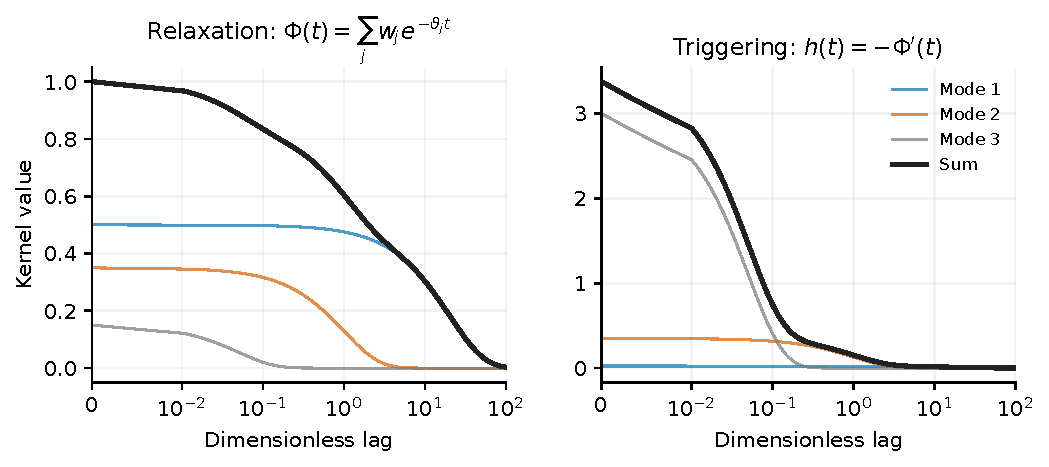
\includegraphics[width=0.95\linewidth]{finite_memory.pdf}
\caption{A dimensionless toy finite mixture with weights $(0.5,0.35,0.15)$ and rates $(0.05,1,20)$. The relaxation $\Phi$ and its negative derivative $h$ weight the same modes differently. Curves are direct evaluations of the displayed finite sums; they are not fits, simulations or an exact Mittag--Leffler kernel.}
\label{fig:finite_memory}
\end{figure}

In the physical model \(w_j\) is dimensionless, \(\vartheta_j\) and \(h\) have inverse-time units, \(\Phi\) is dimensionless, \(\rho\) is stress per unit time, and \(g(M)\) is measured in stress units. The jump \(\vartheta_j\kappa(M)\) has the units of \(U_j\). With no history, the sums in \eqref{eq:finite-X-mild}--\eqref{eq:finite-H-mild} are empty.

\section{The diagnostic model and observation}\label{sec:model_diagnostic}

For diagnostic work, retain a stress relaxation kernel \(\Phi_s\) and a normalized triggering density \(h_e\), initially allowing them to vary separately. Let \((T_i,Q_i)\) denote the accepted event times and their marks. Define the strictly prior cumulative release and excitation sums by
\begin{equation}\label{eq:diagnostic-sums}
G_s(t)=\sum_{0<T_i<t}g(Q_i)\Phi_s(t-T_i),
\qquad
H_e(t)=\sum_{0<T_i<t}\kappa(Q_i)h_e(t-T_i),
\end{equation}
and adopt the diagnostic intensity
\begin{equation}\label{eq:diagnostic-intensity}
\lambda_\eta(t)=B(t)\exp\{-\eta G_s(t)\}+nH_e(t).
\end{equation}

\begin{figure}[htb]
\centering
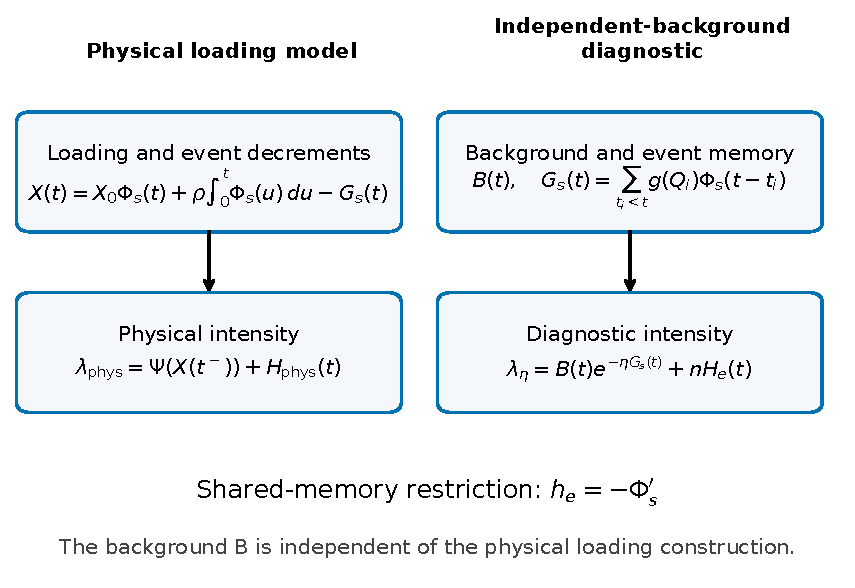
\includegraphics[width=0.95\linewidth]{model_architecture.pdf}
\caption{Physical loading and the independent-background diagnostic answer different questions. The physical model feeds loading through stress; the diagnostic specifies a background and suppresses its contribution by accumulated release. Triggering remains additive. The unit-productivity convention, with $n$ outside $H_e$, applies to the diagnostic.}
\label{fig:model_architecture}
\end{figure}
The baseline \(B(t)\) is deterministic at fixed parameters and specified independently of the stress-kernel family. A useful choice is \(B(t)=\exp\{a+d(2t/T-1)\}\). It is not generated by stress loading or by the marks. The strict inequalities in \eqref{eq:diagnostic-sums} are deliberate: an event is accepted before its mark is drawn, so its own release and productivity cannot enter its intensity.

This section adopts a convention change once and for all: diagnostic productivity is scaled to have unit mean,
\[
\mathbb E_F\kappa(Q)=1,
\]
while the coefficient \(n\) is retained \emph{outside} \(H_e\) in \eqref{eq:diagnostic-intensity}. In the physical model, by contrast, \(n=\mathbb E_F\kappa(M)<1\) is the mean carried by the productivity marks themselves. The diagnostic normalisation removes that mean from the marks and displays it explicitly as a coefficient. This is a bookkeeping convention, not an assertion that realised productivity is one, and it is not used to reinterpret the autonomous physical stability theorem.

The physical exponential link \eqref{eq:physical-link} embeds loading through \(X\): a constant \(\rho\) shifts the physical stress state and therefore changes \(\Psi(X)\). The time-dependent baseline \(B(t)\) in \eqref{eq:diagnostic-intensity} is an independently specified background. It does not replace \(\Psi(X)\) in the autonomous invariant-law theorem; that theorem does not cover externally varying \(B(t)\).

The shared subfamily imposes the identity \(h_e=-\Phi_s'\). This has substantive model content: the instantaneous excitation density is the negative derivative of the same kernel that governs stress relaxation. Consequently the decay of past stress and the contribution of a mark to the future compensator come from one memory structure, including its normalisation. Choices of \(\Phi_s\) and \(h_e\) that do not satisfy this identity define a separate-memory model. Normalization alone does not impose their equality. See \sourcesupp{S22}.

A ground process records only the event times \(T_i\), whereas a marked process records the pairs \((T_i,Q_i)\). The ground law is a projection of the marked law. The event-time contribution to a joint marked likelihood, evaluated using observed past marks, is a different object from the marginal likelihood of times alone. Event times alone generally do not identify \(g\) and \(\kappa\) separately, nor their within-mark dependence, without an additional mark model. Conversely, the marked likelihood includes both ground acceptance probabilities and mark densities. Since marks are fresh after acceptance, past marks enter \eqref{eq:diagnostic-intensity} through the strict sums \eqref{eq:diagnostic-sums}, while a newly drawn mark first affects the future. This observational distinction is essential: marginalizing to times alone and evaluating a joint marked likelihood answer different questions.



The likelihoods studied below condition on a declared starting history. Empty prehistory is a model assumption rather than a statement that no earlier earthquakes occurred. Likewise, a fresh common mark law does not establish completeness or homogeneous measurement of the observed catalogue. Unobserved parents, omitted regions and uncertain magnitudes can change the relationship between the mathematical history and its recorded counterpart. The subsequent identification statements concern the declared complete marked process; their transfer to an earthquake catalogue requires an observation model.
